\begin{blocksection}
\question Let the path sum of any node in the tree be equal to the sum of its label and the labels of all nodes on the path from the root to that node. For example, for the following tree:
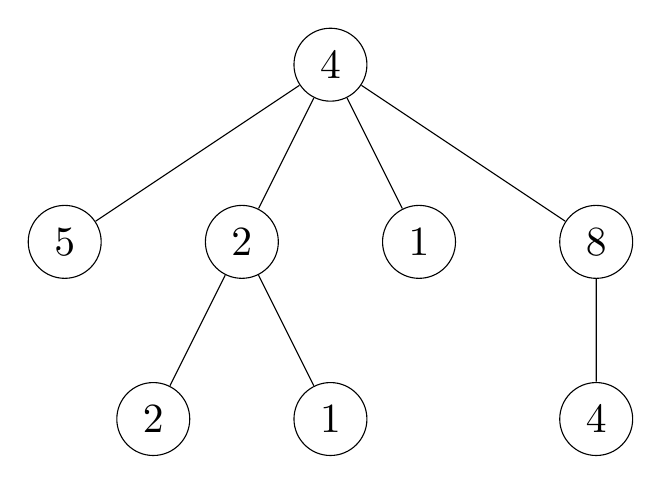
\begin{tikzpicture}[scale=1.5, transform shape]
    \node [circle, draw] (z){$4$}
        child {node [circle, draw] (a) {$5$}}
        child {node [circle, draw] (b) {$2$}
            child {node [circle, draw] (e) {$2$}}
            child {node [circle, draw] (f) {$1$}}
        }
        child {node [circle, draw] (c) {$1$}}
        child {node [circle, draw] (d) {$8$}
            child {node [circle, draw] (g) {$4$}}
        };
\end{tikzpicture}

The path sum of each node in the tree is as follows:

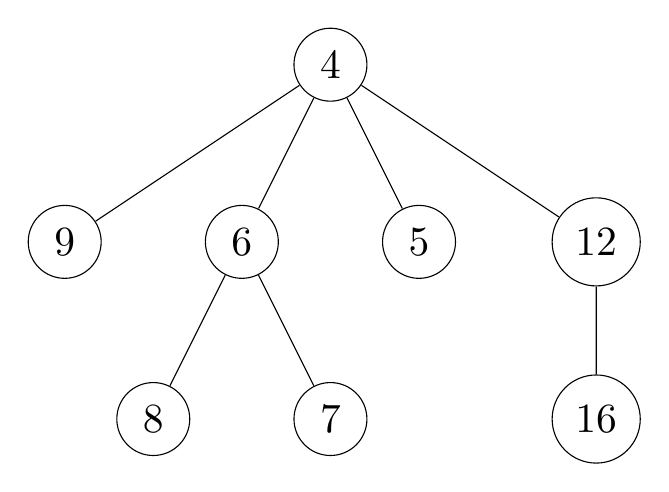
\begin{tikzpicture}[scale=1.5, transform shape]
    \node [circle, draw] (z){$4$}
        child {node [circle, draw] (a) {$9$}}
        child {node [circle, draw] (b) {$6$}
            child {node [circle, draw] (e) {$8$}}
            child {node [circle, draw] (f) {$7$}}
        }
        child {node [circle, draw] (c) {$5$}}
        child {node [circle, draw] (d) {$12$}
            child {node [circle, draw] (g) {$16$}}
        };
\end{tikzpicture}

Write a generator that takes in a Tree object and yields the path sum of each node in the tree. The path sum of a node should be yielded only after the path sum of all of its children have been yielded. (Tangential note: this ordering is called post-order DFS). See doctests.


\begin{lstlisting}
def gen_path_sums(t):
    """
    >>> t = Tree(1, [Tree(2, [Tree(5)]), Tree(3, [Tree(4)])])
    >>> print(list(gen_path_sums(t)))
       	[8, 3, 8, 4, 1] # draw out the tree and check your understanding!
    >>> 
    """    
    for _____________________________
    	for _______________________________
    		_______________________________
    _______________________
\end{lstlisting}
\end{blocksection}

\begin{blocksection}
\begin{solution}[0.5in]
\begin{lstlisting}
def gen_path_sums(t):
    for b in t.branches:
        for branch_sum in gen_path_sums(b):
            yield t.label + branch_sum
    yield t.label
\end{lstlisting}

\end{solution}
\end{blocksection}
